\documentclass{article}
\usepackage{graphicx} % Required for inserting images
\usepackage{enumitem}
\usepackage{xcolor}
\usepackage{listings}
\usepackage{mathtools}
\usepackage{amsmath}
\newcommand{\logicarg}[2]{% \logicarg{<premise>}{<conclusion>}
  \begin{tabular}[t]{@{}l@{}}
    #1 \\ \hline #2
  \end{tabular}%
}

\setlength{\oddsidemargin}{-0.25in}
\setlength{\topmargin}{-0.5in}
\setlength{\headheight}{0cm}
\setlength{\headsep}{0cm}
\setlength{\textheight}{10in}
\setlength{\textwidth}{7in}
\setlength{\topskip}{0cm}

\begin{document}

\noindent\textbf{ComS 472 - PS11 \quad Due: Dec 8, 2024 \quad Name: Aren Ashlock}

\begin{enumerate}

% ------------------------------------- 1 DONE -------------------------------------

\item \textbf{(20 pts)} (Exercise 14.21) Consider the query $\mathbf{P}(Rain|Sprinkler=true, WetGrass=true)$ in the figure below and how Gibbs sampling via uniform choice of nonevidence variables can answer it.

\begin{center}
    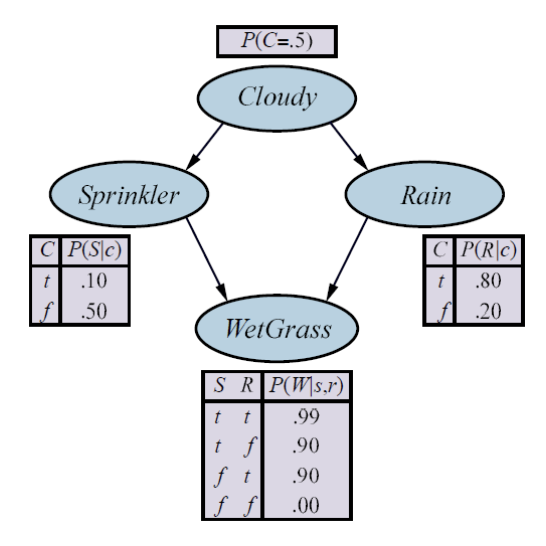
\includegraphics[scale=0.5]{472-PS11-Q1}
\end{center}

\begin{enumerate}[label=($\alph*$)]

    % ----------------------------------- 1a DONE -----------------------------------
   
    \item \textbf{(2 pts)} How many states does the Markov chain for this query have?

    \color{blue}
        4
    \color{black}

    % -------------------------------------------------------------------------------

    % ----------------------------------- 1b DONE -----------------------------------

    \item \textbf{(10 pts)} Calculate the \textit{transition matrix Q} containing the kernel $k(\mathbf{y} \rightarrow \mathbf{y'})$ for every directed edge from, say, a state $\mathbf{y}$ to another state $\mathbf{y'}$ or itself (in the case $\mathbf{y} = \mathbf{y'}$), in the Markov chain. Label the rows and columns of the matrix by the states such that an entry in the matrix corresponds to the probability of a transition from the state given by the row label to the state given by the column label.

    \color{blue}
        $\begin{matrix}
        & (c, r) & (c, \neg r) & (\neg c, r) & (\neg c, \neg r)\\
        (c, r) & 0.6295 & 0.0925 & 0.278 & 0\\
        (c, \neg r) & 0.4075 & 0.1165 & 0 & 0.476\\
        (\neg c, r) & 0.222 & 0 & 0.386 & 0.392\\
        (\neg c, \neg r) & 0 & 0.024 & 0.108 & 0.868\\
        \end{matrix}$
    \color{black}

    % -------------------------------------------------------------------------------

    % --------------------------------- 1c NOT DONE ---------------------------------

    \item \textbf{(2 pts)} What does $Q^2$, the square of the transition matrix, represent?

    \color{blue}
        It represents the probability of starting with the state in the row and ending in the column state after 2 steps.
    \color{black}

    % -------------------------------------------------------------------------------

    % ----------------------------------- 1d DONE -----------------------------------

    \item \textbf{(3 pts)} What about $Q^n$ as $n \rightarrow \infty$?

    \color{blue}
        As $n \rightarrow \infty$, $Q^n$ reaches a stationary distribution which represents the probability of being in a state.
    \color{black}

    % -------------------------------------------------------------------------------

    % ----------------------------------- 1e DONE -----------------------------------

    \item \textbf{(3 pts)} Explain how to do probabilistic inference in a Bayesian network, assuming that $Q^n$ is available. Is this a practical way to do inference?

    \color{blue}
        You can multiply $Q^n$ however many times you need to reach different numbers of steps. And you can do it efficiently by multiplying the newly calculated matrices together to get higher power matrices in less calculations. However, matrix multiplication requires a lot of computation, so I don't think it is very practical.
    \color{black}

    % -------------------------------------------------------------------------------
    
    \end{enumerate}

% ----------------------------------------------------------------------------------

% ------------------------------------- 2 DONE -------------------------------------

\item \textbf{(10 pts)} (Exercise 14.22) This exercise explores the stationary distribution for Gibbs sampling methods.

\begin{enumerate}[label=($\alph*$)]

    % ----------------------------------- 2a DONE -----------------------------------

    \item \textbf{(5 pts)} The convex composition $[\alpha, k_1; 1-\alpha, k_2]$ of two transition kernels $k_1$ and $k_2$ is a transition probability distribution that first chooses one of $k_1$ and $k_2$ with probabilities $\alpha$ and $1-\alpha$, respectively, and then applies whichever is chosen. Prove that if $k_1$ and $k_2$ are in detailed balance with a stationary distribution $\pi$, then their convex composition is also in detailed balance with $\pi$.

    \color{blue}
        $\pi(\textbf{x})(\alpha k_1(\textbf{x} \rightarrow \textbf{x'}) + (1-\alpha)k_2(\textbf{x} \rightarrow \textbf{x'})) = \pi(\textbf{x'})(\alpha k_1(\textbf{x'} \rightarrow \textbf{x}) + (1-\alpha)k_2(\textbf{x'} \rightarrow \textbf{x}))$\\
        $\alpha \pi(\textbf{x}) k_1(\textbf{x} \rightarrow \textbf{x'}) + (1-\alpha) \pi(\textbf{x}) k_2(\textbf{x} \rightarrow \textbf{x'}) = \pi(\textbf{x'})(\alpha k_1(\textbf{x'} \rightarrow \textbf{x}) + (1-\alpha)k_2(\textbf{x'} \rightarrow \textbf{x}))$\\
        \textbf{We know that $k_1$ and $k_2$ are in detailed balance with $\pi$, so apply that rule...}\\
        $\alpha \pi(\textbf{x'}) k_1(\textbf{x'} \rightarrow \textbf{x}) + (1-\alpha) \pi(\textbf{x'}) k_2(\textbf{x'} \rightarrow \textbf{x}) = \pi(\textbf{x'})(\alpha k_1(\textbf{x'} \rightarrow \textbf{x}) + (1-\alpha)k_2(\textbf{x'} \rightarrow \textbf{x}))$\\
        $\pi(\textbf{x'})(\alpha k_1(\textbf{x'} \rightarrow \textbf{x}) + (1-\alpha) k_2(\textbf{x'} \rightarrow \textbf{x})) = \pi(\textbf{x'})(\alpha k_1(\textbf{x'} \rightarrow \textbf{x}) + (1-\alpha)k_2(\textbf{x'} \rightarrow \textbf{x}))$
    \color{black}

    % -------------------------------------------------------------------------------

    % ----------------------------------- 2b DONE -----------------------------------

    \item \textbf{(5 pts)} Prove that if each of $k_1$ and $k_2$ has $\pi$ as its stationary distribution, then the sequential composition $k = k_2 \circ k_1$ defined by

    \begin{equation*}
        (k_2 \circ k_1)(\mathbf{x} \rightarrow \mathbf{x'}) = \sum_{\mathbf{x''}} k_1(\mathbf{x} \rightarrow \mathbf{x''})k_2(\mathbf{x''} \rightarrow \mathbf{x'})
    \end{equation*}

    also has $\pi$ as its stationary distribution.

    \color{blue}
        $\sum_{\mathbf{x}}\pi(\mathbf{x})(k_2 \circ k_1)(\mathbf{x} \rightarrow \mathbf{x'}) = \sum_{\mathbf{x}}\pi(\mathbf{x})\sum_{\mathbf{x''}} k_1(\mathbf{x} \rightarrow \mathbf{x''})k_2(\mathbf{x''} \rightarrow \mathbf{x'})$\\
        $\pi(\mathbf{x'}) = \sum_{\mathbf{x''}} k_2(\mathbf{x''} \rightarrow \mathbf{x'}) \sum_{\mathbf{x}}\pi(\mathbf{x}) k_1(\mathbf{x} \rightarrow \mathbf{x''})$\\
        $\pi(\mathbf{x'}) = \sum_{\mathbf{x''}} k_2(\mathbf{x''} \rightarrow \mathbf{x'}) \pi(\mathbf{x''})$\\
        $\pi(\mathbf{x'}) = \sum_{\mathbf{x''}} \pi(\mathbf{x''}) k_2(\mathbf{x''} \rightarrow \mathbf{x'})$\\
        $\pi(\mathbf{x'}) = \pi(\mathbf{x'})$
    \color{black}

    % -------------------------------------------------------------------------------
    
    \end{enumerate}

% ----------------------------------------------------------------------------------

\end{enumerate}
\end{document}